\chapter{Speichertechnologien}

In diesem Kapitel werden die Energiespeicher für Stadtbusse betrachtet. Wie im vorigen Kapitel werden zunächst die Technologien erläutert. Die Parameter sind aufgeteilt in Parameter, die direkt bewertet werden und Eingabewerte für die Simulation. In Abschnitt \ref{vergleichstabellen_speichertechnologien} ab Seite \pageref{vergleichstabellen_speichertechnologien} sind die Werte aufgelistet. \marginpar{ÜBERARBEITEN (für Parameterliste)}

Im Gegensatz zu den Ladesystemen ist die Produktvielfalt der Speichertechnologien nahezu unbegrenzt. Von daher werden hier nur Technologien aufgelistet, die bereits in elektrischen Stadtbussen eingesetzt wurden. Die Daten stammen von aktuell erhältlichen Produkten für elektrische Straßenfahrzeuge.

\section{Untersuchte Technologien}
Im folgenden Abschnitt werden die Grundlagen und die Einsatzgeschichten der verschiedenen Speichertechnologien kurz erläutert. Die Technologien sind nach dem genutzten physikalischen Effekt aufgeteilt~\cite{Sterner:2014}[S. 35f]. Im realen Betrieb werden manchmal auch Kombinationen von verschiedenen Speichertechnologien eingesetzt, um dem hohen Leistungsbedarf beim Anfahren und bei der Bremsenergierückgewinnung gerecht zu werden.

\subsection{Mechanisch – Schwungradspeicher}
In Bussen kann mechanische Energie mit einem Schwungrad gespeichert werden\footnote{Es gibt auch Prototypen von Pressluftspeichern in kleineren Fahrzeugen, in Bussen werden sie jedoch nur als Teil eines Hybridantriebs eingesetzt und hier nicht weiter betrachtet~\cite{Sebastian-Naumann:2014}[S. 14].}. Die Energieübertragung erfolgt durch eine elektrische Motor- und Generatoreinheit. Moderne Schwungräder werden aus gewickelten Karbonfasern hergestellt und in Vakuumgehäusen magnetisch gelagert. So werden Drehzahlen von bis zu 40.000~min\textsuperscript{-1} und sehr geringe Reibungsverluste erreicht~\cite{993788}. Um die Sicherheit der Passagiere zu gewährleisten muss das Gehäuse im Falle eines berstenden Schwungrades die gesamte gespeicherte Energie innerhalb von Sekundenbruchteilen aufnehmen können, ohne selbst zu bersten. Dies erfordert sehr schwere Gehäuse, die die spezifische Energie und Leistung des tatsächlichen Systems stark reduzieren.

Der Schwungradspeicher wurde in den fünfziger Jahren im Gyrobus im schweizerischen Yverdon auf einer acht Kilometer langen Linie erprobt. Die Strecke wurde erfolgreich zurückgelegt, die damalige Technologie war jedoch sehr wartungsaufwändig und weniger effizient als ein Oberleitungsbus. Aktuell wird der Schwungradspeicher nur als Teil eines hybriden Antriebsstrangs eingesetzt und daher in dieser Arbeit nicht weiter betrachtet~\cite{tub_aleph001746639}[S. 216].

\subsection{Elektrisch – Kondensator}
Der Kondensator ist ein rein elektrischer Energiespeicher. Im klassischen Plattenkondensator werden zwei durch ein festes Dielektrikum getrennte Platten elektrisch aufgeladen, die Ladung kann später in Strom umgewandelt werden. Kondensatoren haben eine hohe spezifische Leistung, aber eine sehr geringe spezifische Energie.

In Bussen werden deshalb sogenannte Superkondensatoren verwendet, die statt eines festen Dielektrikums ein Elektrolyt (meist eine Salz-Wasser-Lösung) verwenden. Die im Elektrolyt gelösten Ionen werden von der geladenen Platte angezogen, können sie jedoch aufgrund der umgebenden Wasserschicht nicht erreichen (siehe Abbildung \ref{abb_doppelschicht}). Da der Abstand zwischen Platte un Ionen extrem klein ist, entsteht eine sehr hohe elektrische Kapazität. Eine weitere Kapazitätssteigerung wird durch die Einlagerung von einigen Elektronen des Elektrolyts in die Leiterplatten erreicht~\cite{Sterner:2014}[S. 167f].

\begin{figure}\centering
	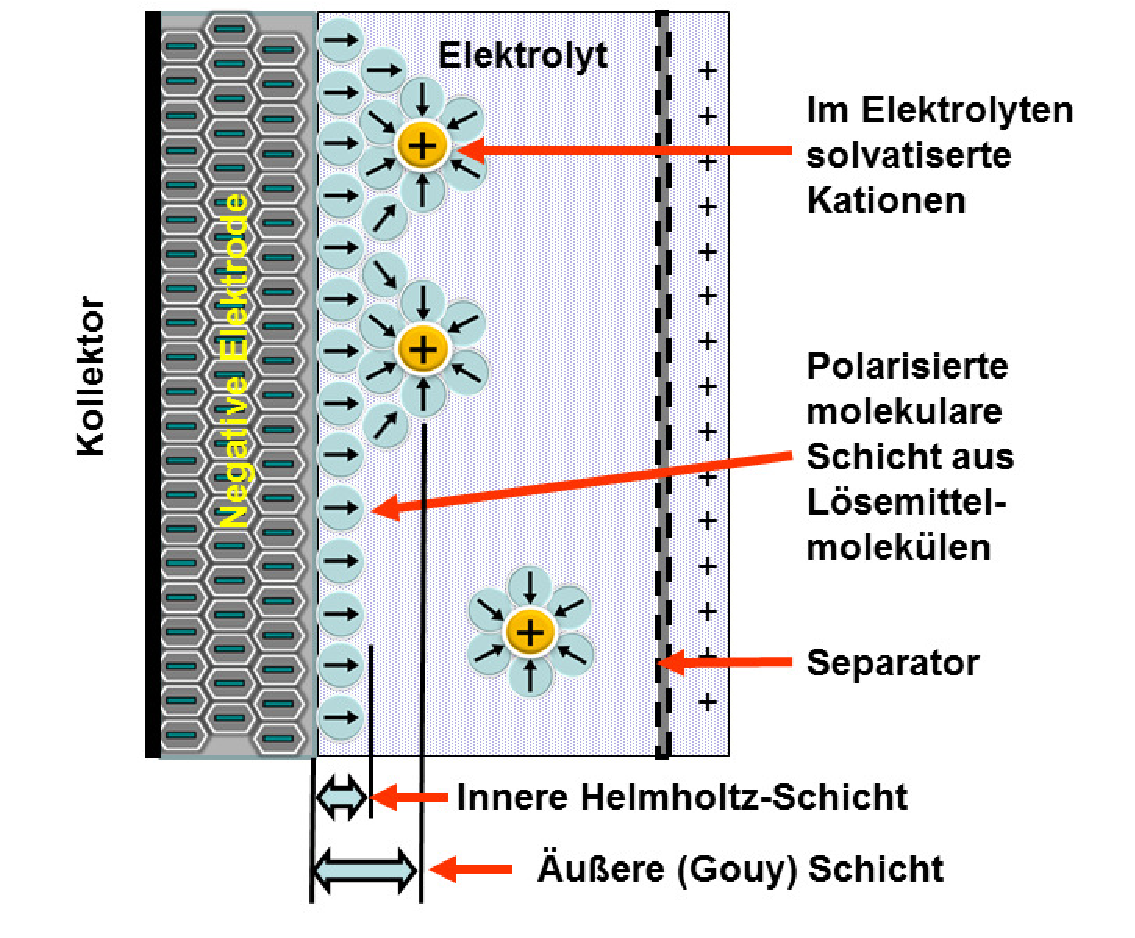
\includegraphics[width=\myFigureStandardWidth]{Doppelschicht-Prinzipdarstellung}
	\caption[Prinzipdarstellung eines Superkondensators]{Prinzipdarstellung eines Superkondensators. Quelle: Elcap (Eigenes Werk) CC BY-SA 3.0, via Wikimedia Commons}
	\label{abb_doppelschicht}
\end{figure}

In Shanghai werden Busse mit dieser Technologie seit 2008 im Linienverkehr eingesetzt. Daneben werden Superkondensatoren für kurzzeitige Einsätze mit hohem Leistungsbedarf, zum Beispiel zur Bremsenergierückgewinnung oder zur Überbrückung stromloser Stellen in Trolleybussen eingesetzt~\cite{Barminer-Busgesellschaft:2012}.

Die spezifische Energie von Superkondensatoren reicht aktuell nicht für ein Aufladen an den Endhaltestellen aus. Stattdessen müssen auch Unterwegshaltestellen zu Ladestationen ausgebaut werden. Aufgrund des hohen Infrastrukturbedarfs werden Superkondensatoren nicht weiter betrachtet.

\subsection{Elektrochemisch – Batterie} %TODO: Besser
Eine Batterie ist ein elektrochemischer Energiespeicher. An den Klemmen besteht eine elektrische Spannung, die direkt abgerufen werden kann. Innerhalb der Batterie besteht ein Ungleichgewicht zwischen den elektrischen Ladungen von zwei Elektroden, die durch ein Elektrolyt getrennt sind. Durch den Elektrolyt können nur Ionen, aber keine Elektronen wandern, von daher wandern die Elektronen durch den Verbraucher von Klemme zu Klemme, sobald der Stromkreis geschlossen wird.

Es wird unterschieden in Primärbatterien, in denen die Reaktion nicht umkehrbar ist und wiederaufladbaren Batterien, sogenannten Sekundärbatterien. In dieser Arbeit werden nur Sekundärbatterien betrachtet\footnote{Die Begriffe Batterie, Akkumulator und Akku werden hier austauschbar verwendet.}, die für den Einsatz in Fahrzeugen geeignet sind.

Die Spannung einer einzelnen Batteriezelle ist durch die verwendeten chemischen Elemente begrenzt~\cite{Sterner:2014}[S. 202f]. Deshalb bestehen sämtliche Batterien für elektrische Fahrzeuge aus einer Parallelschaltung einzelner Zellen, mit der eine höhere Spannung erreicht wird.

Die Bauformen sind sehr unterschiedlich, meist werden jedoch gewickelte oder ineinander geschachtelte, flache Elektroden verwendet um die Oberflächen und damit die Stromstärke zu maximieren~\cite{Sterner:2014}[S. 209ff].

\subsubsection{Wärmeverluste} \label{sec_waermeverluste}
In einer Batterie treten sowohl reversible als auch irreversible thermodynamische Prozesse auf. Die an den Elektroden ablaufenden Reaktionen sind je nach Materialpaarung und Reaktionsrichtung endotherm oder exotherm. Die reversible Erwärmung kann über die Summe der Entropieänderungen an beiden Elektroden berechnet werden~\cite{KiehneBattery}[S. 21ff].
\begin{equation}\label{gl_entropie}
	Q_{rev}=T(\Delta S_{Kat.~Reakt.} + \Delta S_{An.~Reakt.}) \frac{I}{nF}	
\end{equation}
In Gleichung \ref{gl_entropie} ist $I$ der Strom, $n$ die Anzahl der Elektronen pro Reaktion und $F$ die Faradaykonstante. 

Daneben gibt es einen irreversiblen Wärmeverlust, dessen Größe durch den Innenwiderstand bestimmt ist. Im Innenwiderstand $R_i$ werden die Widerstände von Elektroden, Elektrolyt und der irreversible Anteil der Zellenreaktion zusammengefasst.
\begin{equation}\label{gl_innenwiderstand}
Q_{irr}=-I^2\cdot R_i
\end{equation}

Das thermische Verhalten wir durch die Summe der reversiblen und irreversiblen Wärmeentwicklung beschrieben. Der reversible Anteil hängt linear vom Strom ab, der irreversible quadratisch. Für niedrige Ströme kann der reversible Anteil den irreversiblen übertreffen, das heißt die Batterie kann sich bei langsamen Laden oder Entladen \emph{abkühlen}. Bei hohen Strömen überwiegt der irreversible Anteil, bei Lithium-Ionen Akkus entspricht der reversible Anteil bei einer 1$C$-Entladung maximal 50\% des irreversiblen Anteils~\cite{Viswanathan20103720}.


\subsubsection{Blei-Säure}
Der Blei-Säure-Akkumulator besteht aus zwei Bleielektroden in einer Schwefelsäurelösung. Vor dem ersten Aufladen bildet sich an beiden Elektronen Bleisulfat ($PbSO_4$). Die Elektrodengleichungen sind in Tabelle \ref{Pb} auf Seite \pageref{Pb} aufgeführt~\cite{KiehneBattery}[S. 50].

\begin{table}\centering
	\begin{tabularx}{\linewidth}{XrcX}
		\toprule
		&                       $geladen$ & $\rightleftarrows$ & $entladen$             \\
		Negative Elektrode & $PbO_2 + H_2SO_4 + 2H^+ + 2e^-$ & $\rightleftarrows$ & $PbSO_4 + 2H_2O$       \\
		Positive Elektrode &                $Pb + H_2SO_4$ & $\rightleftarrows$ & $PbSO_4 + 2H^+ + 2e^-$ \\ \midrule
		Zellenreaktion     &         $Pb + PbO_2 + 2H_2SO_4$ & $\rightleftarrows$ & $2PbSO_4 + 2H_2O$      \\ \bottomrule
	\end{tabularx}
	\caption{Elektrodengleichungen der Blei-Säure-Batterie}
	\label{Pb}
\end{table}

Im Gegensatz zu den meisten anderen Batterien transportiert hier der Elektrolyt nicht nur die Ionen, sondern ist selbst an der Reaktion beteiligt.

Im geladenen Zustand wird das enthaltene Wasser elektrolytisch zu Wasserstoff und Sauerstoff zerlegt. Dieser Wasserverlust muss durch periodisches Nachfüllen oder Rekombination der Gase zu Wasser ausgeglichen werden. Vorteil der Gasentwicklung ist, dass so durch Überladen die Spannungen verschiedener Zellen angeglichen werden können, da die Energie des Überladevorgangs in die Wasserspaltung geführt wird~\cite{tub_aleph001746639}[S. 182].

Der Blei-Säure-Akkumulator ist eine der ältesten wiederaufladbaren Batterietechnologien und wurde in allen frühen Elektrobussen eingesetzt, zum Beispiel im weltweit ersten Batteriebus, der ab 1900 in Berlin auf der Strecke Anhalter Bahnhof – Stettiner Bahnhof (heute: Nordbahnhof)~\cite{Risch:1957}[S. 8f].

Heutzutage ist die Verwendung von Bleiakkus auf Gabelstapler und andere Fahrzeuge außerhalb des Straßenverkehrs begrenzt. In dieser Arbeit wird dennoch der Bleiakku \textsc{Panasonic EC-FV1260} betrachtet um aufzuzeigen, wie weit die Technologie in den vergangen 40 Jahren fortgeschritten ist.

\subsubsection{Nickel-Cadmium}
Die Elektroden bestehen aus Nickelhydroxid und Cadmiumhydroxid in einem alkalischen, wässrigen Elektrolyt, dass nicht an der Reaktion beteiligt ist, sondern nur dem Ionentransport dient. Die Reaktionsgleichungen sind in Tabelle \ref{NiCd} aufgeführt~\cite{Sterner:2014}[S.233].

\begin{table}\centering
	\begin{tabularx}{\linewidth}{XrcX}
		\toprule
		&               $geladen$ & $\rightleftarrows$ & $entladen$             \\
		Negative Elektrode &            $Cd + 2OH^-$ & $\rightleftarrows$ & $Cd(OH)_2 + 2e^-$      \\
		Positive Elektrode & $2NiO(OH) + 2H_2O + 2e^-$ & $\rightleftarrows$ & $2Ni(OH)_2 + 2OH^-$    \\ \midrule
		Zellenreaktion     &   $Cd + 2NiO(OH) + 2H_2O$ & $\rightleftarrows$ & $Cd(OH)_2 + 2Ni(OH)_2$ \\ \bottomrule
	\end{tabularx}
	\caption{Elektrodengleichungen der Nickel-Cadmium-Batterie}
	\label{NiCd}
\end{table}

Wie bei Blei-Säure-Batterien wird der Elektrolyt in Wasserstoff und Sauerstoff zerlegt. Es sind offene Bauformen und geschlossene Bauformen mit interner Rekombination vorhanden.

Die Nickel-Cadmium-Batterie weist eine weit höhere spezifische Energie als die Blei-Säure-Batterie auf, wird jedoch in elektrischen Bussen nicht verwendet und daher hier auch nicht weiter betrachtet. \marginpar{Warum? Wirklich?}

\subsubsection{Nickel-Metallhydrid}
Die Nickel-Metalhydridbatterie verwendet wie die Nickel-Cadmiumbatterie eine Nickel(oxy)hydroxidelektrode und einen alkalischen Elektrolyt. Der Unterschied ist, das hier statt giftigem Cadmium(hydroxid) in der negativen Elektrode Metall eingesetzt wird, in dem $H^+$-Ionen zu Wasserstoff reduziert und eingelagert werden. Dieser Hydrierung genannte Vorgang tritt in vielen verschiedenen Metallen und Legierungen auf. In diesen Batterien wird meist eine Legierung aus seltenen Erden und Nickel verwendet~\cite{KiehneBattery}[S. 85ff]. Die Reaktionsgleichungen sind in Tabelle \ref{NiMH} aufgeführt~\cite{Sterner:2014}[S. 245].

\begin{table}\centering %TODO: Rahmen für Tabellen
	\begin{tabularx}{\linewidth}{XrcX}
		\toprule
		&              $geladen$ & $\rightleftarrows$ & $entladen$        \\
		Negative Elektrode &          $M(H) + OH^-$ & $\rightleftarrows$ & $M + H_2O + e^-$  \\
		Positive Elektrode &   $NiO(OH) + H_2O + e^-$ & $\rightleftarrows$ & $Ni(OH)_2 + OH^-$ \\ \midrule
		Zellenreaktion     & $M(H) + NiO(OH) + 2H_2O$ & $\rightleftarrows$ & $M + Ni(OH)_2$    \\ \bottomrule
	\end{tabularx}
	\caption{Elektrodengleichungen der Nickel-Metallhydrid-Batterie}
	\label{NiMH}
\end{table}

Da die Hydrierung bei einem Druck von bis zu 10 Bar stattfindet, gibt es nur geschlossene Bauformen. Der Nickel-Metallhydrid-Akku wird in mehreren Hybridfahrzeugen verwendet, zum Beispiel im Toyota Prius. Nickel-Metallhydrid-Akkus sind inzwischen teurer als vergleichbare Lithium-Ionen-Akkus~\cite{Schimke:2012}[S. 33]. Von daher werden sie hier nicht weiter betrachtet.

\subsubsection{Lithium-Ionen}
In Lithium-Ionen-Akkus erfolgt der Ladungstransfer durch $Li^+$-Ionen, die durch ein Elektrolyt aus Lithiumsalzen in organischen Lösungsmitteln wandern. Der Elektrolyt ist häufig in ein Polymer eingelagert. Das so entstandene Gel dient sowohl als Elektrolyt als auch zur mechanischen Separation der Elektroden\footnote{Es wird auch an einphasigen, festen Polymerelektrolyten geforscht, mit deren geringer Dicke eine hohe Energiedichte erreicht werden könnte. Diese Technologie wird jedoch noch nicht kommerziell eingesetzt.}~\cite{xu2004nonaqueous}. Im Gegensatz zu den anderen Batterietypen, bei denen das Elektrodenmaterial oxidiert und reduziert wird, wandert hier das Metall selber von Elektrode zu Elektrode. Reine Lithiumelektroden würden sich auflösen und dadurch ihre Form verlieren. Von daher werden für positive und negative Elektroden verschiedene Materialien verwendet, in denen die Lithiumionen eingelagert werden~\cite{KiehneBattery}[S. 408, 440ff]. 

\paragraph{Geschichtete Oxide}

\begin{figure}\centering
	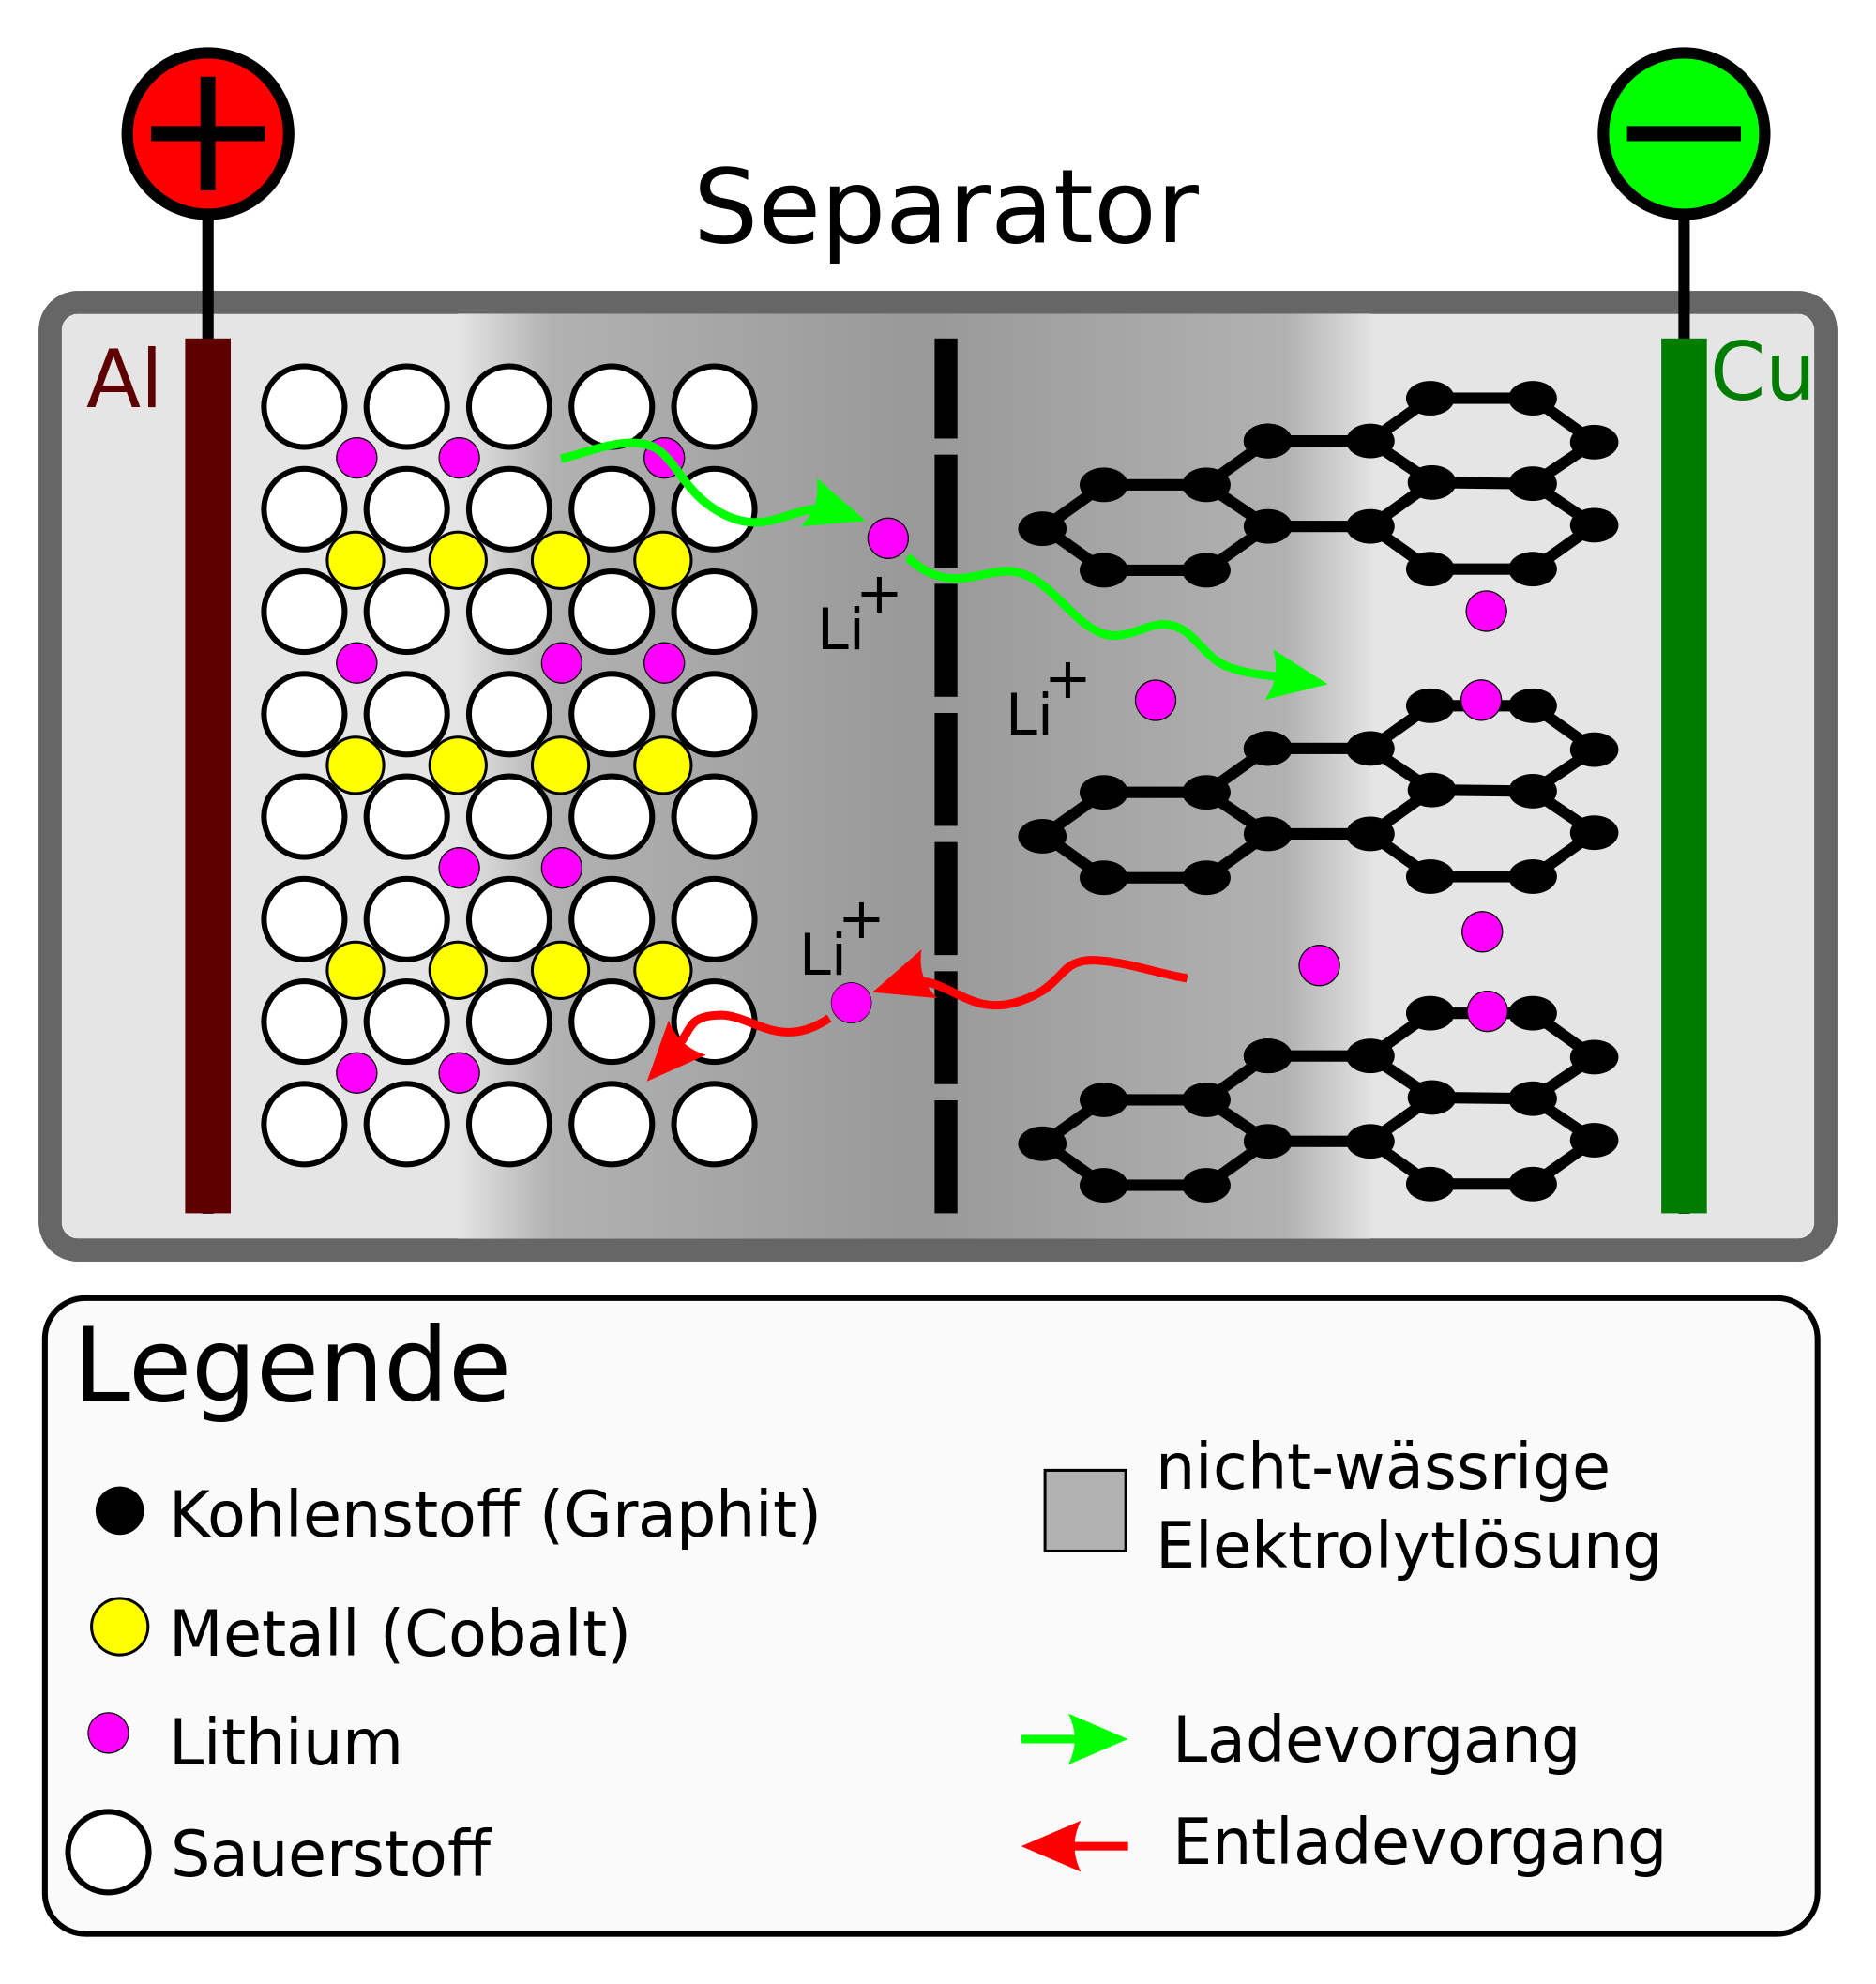
\includegraphics[width=\myFigureStandardWidth]{LiCoO2}
	\caption[Prinzipdarstellung eines Lithium-Ionen-Akkus]{Prinzipdarstellung eines Lithium-Ionen-Akkus mit Kobaltoxid in der positiven Elektrode. Quelle: Cepheiden (Eigenes Werk) CC BY-SA 2.0, via Wikimedia Commons} %TODO: Zitierweise
	\label{abb_LiCoO2}
\end{figure}

In kleinen und mittelgroßen Akkus werden meist positive Elektroden aus Lithium-Metalloxiden verwendet. Diese haben eine kubische Kristallstruktur. Das Lithium wird zwischen den Sauerstoffatomen eingelagert. Positive Elektroden aus $LiCoO_2$ werden seit den 90er Jahren in kommerziellen Lithiumakkus verwendet. Daneben sind auch Lithium-Manganoxide und Mischungen von Lithium-Nickel- und Lithium-Kobaltoxid gebräuchlich, mit denen man günstigere Akkus auf Kosten der spezifischen Energie herstellen kann~\cite{whittingham2004lithium}. %TODO: Welche Busse?

Die negative Elektrode besteht in allen Fällen aus Graphit. Die Lithiumionen werden zwischen den verschiedenen Schichten der Graphitkristalle eingelagert. Es werden verschiedene Größen von Graphitkristallen und auch andere Modifikationen von Kohlenstoff verwendet~\cite{Sterner:2014}[S. 252]. Ein Lithium-Kobaltoxid-Akku ist in Abbildung \ref{abb_LiCoO2} schematisch dargestellt.

Tesla Motors verwendet im Gegensatz zu anderen Herstellern von Elektrofahrzeugen keine speziellen Batterien, sondern generische 18650-Zellen, wie sie in Laptops verwendet werden\marginpar{Beleg!}. In dieser Arbeit wird die Batterie \textsc{NCR18650B} von \textsc{Panasonic} als Beispiel für "`klassische"' Lithium-Ionen-Akkus betrachtet.

\paragraph{Lithium-Eisenphosphat}
Lithium-Eisenphosphat ($LiFePO_4$) ist ein neues Material für die positive Elektrode. Die theoretische spezifische Energie ist ähnlich der von geschichteten Oxiden, aktuell wird jedoch nur eine niedrigere spezifische Energie erreicht~\cite{Tie201382}. In der negativen Elektrode wird Graphit verwendet. Aufgrund des niedrigen Preises von Eisen sind diese Batterien gut für elektrische Fahrzeuge geeignet und werden zum Beispiel in den elektrischen Bussen von \textsc{BYD} verwendet~\cite{bydSpecs}.

In dieser Arbeit werden zwei Lithium-Eisenphosphat-Akkus betrachtet. Es handelt sich jeweils um Zellen mit hoher Kapazität für den Einsatz in Elektrofahrzeugen. Die Batterie \textsc{EV 45 Ah} von \textsc{European Batteries} ist auf hohe spezifische Energie auf Kosten der Leistung ausgelegt. Im Gegensatz ist die Batterie \textsc{ePLB F 14 AH} auf eine hohe spezifische Entladeleistung ausgelegt.

\paragraph{Lithium-Titanat}
Anders als die vorigen Materialien ist Lithium-Titanat ($Li_4Ti_5O_{12}$) kein Material für die positive Elektrode, sondern ersetzt das Graphit in der negativen Elektrode und wird meist in Kombination mit $LiCoO_2$ eingesetzt. Diese Technologie bietet eine niedrigere spezifische Energie, dafür aber eine weit höhere spezifische Lade- und Entladeleistung~\cite{veneri2012charging}. Damit ist sie insbesondere für Stadtbusse mit Gelegenheitsladung interessant und wird im Berliner Elektrobus-Projekt sowie von \textsc{Proterra} in elektrischen Stadtbussen eingesetzt~\cite{protCat}.

In dieser Arbeit wird die \textsc{primove}-Batterie betrachtet, die im Berliner Elektrobus zum Einsatz kommt.

\subsubsection{Natrium-Nickelchlorid}
Die Natrium-Nickelchloridbatterie (auch als ZEBRA-Batterie bekannt) ist eine Hochtemperaturbatterie. Sie verwendet als Elektrolyt feste Aluminiumkeramik, die nur für $Na^+$-Ionen durchlässig ist. Die Elektroden bestehen aus flüssigem Kochsalz und Nickel, der ebenfalls in flüssigem Kochsalz gelagert ist. Die Reaktionsgleichungen sind in Tabelle \ref{ZEBRA} aufgeführt~\cite{KiehneBattery}[S. 257ff].

\begin{table}\centering %TODO: RICHTIG
	\begin{tabularx}{\linewidth}{XrcX}
		\toprule
		&       $geladen$ & $\rightleftarrows$ & $entladen$           \\
		Negative Elektrode & $NiCl_2 + 2e^-$ & $\rightleftarrows$ & $2Cl^- + 2Na^+ + Ni$ \\
		Positive Elektrode &           $2Na$ & $\rightleftarrows$ & $2e^-$               \\ \midrule
		Zellenreaktion     &  $2Na + NiCl_2$ & $\rightleftarrows$ & $Ni + 2NaCl$ \\ \bottomrule
	\end{tabularx}
	\caption{Elektrodengleichungen der Natrium-Nickelchlorid-Batterie}
	\label{ZEBRA}
	%TODO: Formeln
\end{table}
\marginpar{Formeln in \ref{ZEBRA}}

Damit das Kochsalz flüssig bleibt, muss die Batterie permanent geheizt werden, es werden immer ca. 100W pro 20kWh Kapazität zum Heizen benötigt. Im Gegenzug besitzt dieser Batterietyp eine hohe Lebensdauer und Leistungsdichte. In Kalifornien wurde ein Schulbus mit dieser Batterietechnologie erprobt~\cite{Electric-Transportation-Department:2004}. Aufgrund ihrer geringen Lebensdauer werden sie nicht in Fahrzeugen eingesetzt und hier nicht weiter betrachtet~\cite{Schimke:2012}[S. 24].

\section{Parameter}
Die Bewertung der Speichersysteme erfolgt anhand der Ausgabedaten einer Verbrauchssimulation. In diesem Abschnitt werden die Kenndaten der Energiespeicher erläutert. Sie sind Eingangsdaten der Verbrauchssimulation. Die Verbrauchssimulation und ihre Ausgabedaten werden in Kapitel \ref{chap4} erläutert.

Die Entlade- und Ladekurven der Batterien sind in Anhang \ref{an_Datenblaetter} zu finden. Wenn keine Kurve für das Verhältnis von Ladestrom zu Ladezustand verfügbar war, wurde sie mit einer simulierten CC-CV-Aufladung ermittelt.
\begin{description}
	\item[Entladekurve] Graph von Spannung und Kapazität für verschiedene Ströme.
	\item[Aufladung] Graph von Ladestrom in Abhängigkeit vom Ladezustand.
\end{description}
Die folgenden Parameter sind in Tabelle \ref{vergleichstabellen_speichertechnologien} aufgelistet:
\begin{description}
	\item[Spannung $U$] Die Nennspannung laut Datenblatt.\\
	Einheit: $V$
	\item[Kapazität $Q$] Die Nennkapazität der Batterie\footnote{Diese physikalische Größe hieße richtig \emph{Ladung}. In der Literatur wird jedoch meist das Wort \emph{Kapazität} verwendet.}.\\
	Einheit: $Ah$
	\item[Maximaler Entladestrom $I$] Es wird er maximale Pulsstrom für einen ca. 30-sekündigen Stromstoß verwendet.\\
	Einheit: $A$
	\item[Innenwiderstand $R$] Sollte kein Innenwiderstand dokumentiert sein, wird als Schätzwert 1\% der Nennleistung verwendet.\\
	Einheit: $m\Omega$
	\item[Gewicht] Einheit: $kg$
	\item[Volumen] Das Packvolumen einer Batterieeinheit. Bei Zylindrischen Zellen Beispielsweise $\frac{2\sqrt{3}}{\pi} \cdot V_{Zelle}$.\\
	Einheit: $l$
	\item[Wärmekapazität $c_p$] Die spezifische Wärmekapazität einer Batterie dieses Typs nach Pesaran~\cite{pesaran2001battery}.\\
	Einheit: $\frac{kJ}{kg\cdot K}$
	\item[Höchsttemperatur] Wenn sich Lade- und Entladetemperatur unterscheiden wird der jeweils kleinere Wert verwendet.\\
	Einheit: $^{\circ}C$
\end{description}

\begin{table}\centering
	\begin{tabularx}{\textwidth}{XXrrrrrrrr}
		\toprule
		Kurzname & Chemie           & U   &    Q &   I &         R &   Gew. &   Vol. &                  $c_p$ &       Temp. \\
		         &                  & $V$ & $Ah$ & $A$ & $m\Omega$ &   $kg$ &    $l$ & $\frac{kJ}{kg\cdot K}$ & $^{\circ}C$ \\ \midrule
		18650    & $LiNi_xCo_xAl_x$ & 3,6 & 3,35 & 7,2 &       1,8 & 0,0485 & 0,0176 &                  0,795 &          45 \\
		Bleiakku & $PbSO_4$         & 12,0  &   43 & 180 &       3,5 &     21 &    7,9 &                  0,660 &          50 \\
		LiTiO    & $Li_4Ti_5O_{12}$ & 3,7 &   42 & 133 &       1,2 &      2 &    1,4 &                  0,795 &          55 \\
		LFP-HE   & $LiFePO_4$       & 3,2 &   45 & 160 &       2,0 &   0,99 &    0,6 &                  0,795 &          45 \\
		LFP-HP   & $LiFePO_4$       & 3,2 &   14 & 140 &       5,0 &   0,38 &    0,3 &                  0,795 &          45 \\ \bottomrule
	\end{tabularx}
	\caption{Parameter der Batterien}
	\label{vergleichstabellen_speichertechnologien}
\end{table}
